\chapter{先天免疫与炎症}\label{ch:b3:innate-immunity}

皮下的一根木刺带入了一万个细菌，它们
每半小时便倍增一次。几分钟之内，周围血管扩张并渗漏；
一小时之内，最早的\omterm{def:b3:innate-immunity:innate}{中性粒细胞}已挤出
血管，正沿化学信号的踪迹朝入侵者爬行；
一天之内，局部发红、\omterm{prop:b3:innate-immunity:systemic}{发热}、肿胀、疼痛——
即两千年前塞尔苏斯列出的\omterm{def:b3:innate-immunity:inflammation}{炎症}四大症状——而
细菌已被杀灭，被一些细胞吞噬，这些细胞
此前从未接触过它们，却能将其识别为异物。这就是\omterm{def:b3:innate-immunity:innate}{先天免疫}：
每种动物都具有的防御机制，在感染之前即已就绪，由基因组编码
而非后天习得。它反应迅速，多数入侵者由其消灭，
并向下一章所讲的、较慢的后天习得性免疫发出信号：有东西需要学习。
其过度反应——如脓毒性休克、慢性\omterm{def:b3:innate-immunity:inflammation}{炎症}，
以及自身\omterm{def:b3:innate-immunity:inflammation}{炎症}性疾病所致的\omterm{prop:b3:innate-immunity:systemic}{发热}——
与其成功同样发人深省。

\section{层次与细胞}

\begin{definition}[先天免疫]\label{def:b3:innate-immunity:innate}
\index{先天免疫}\index{中性粒细胞}\index{巨噬细胞}\index{树突状细胞}\index{自然杀伤细胞}\index{屏障}
\emph{先天免疫}是指在任何接触之前即已存在的
一组防御机制，由不发生重排的种系基因编码，
识别微生物的保守特征而非特定个体，
在数分钟至数小时内起作用，并（有所保留地）不具记忆。其
第一层是\emph{屏障}：皮肤的角质、黏液与
气道\omterm{def:b3:cytoskeleton-motility:cilia}{纤毛}、胃酸，以及尿液的冲刷作用，
泪液的冲刷，以及能切割\omterm{def:b3:bacteriology:envelope}{肽聚糖}的溶菌酶，
\emph{抗菌肽}（防御素、cathelicidins）能刺穿
微生物的膜，以及占据
生态位的\omterm{def:b3:microbiomes:symbiosis}{共生}\omterm{def:b3:microbiomes:symbiosis}{微生物组}（见\cref{ch:b3:microbiomes}）。其细胞除最后一类外都来自髓系：
\emph{中性粒细胞}占血液白细胞的 \qty{60}{\%}，
每日生成 $10^{11}$ 个，寿命一天，最先抵达并
是杀灭细菌的主力；\emph{巨噬细胞}为长寿的
组织驻留细胞，分布于各组织（肝脏中的库普弗细胞、脑中的小胶质细胞、
肺中的肺泡巨噬细胞），负责吞噬、清理并
发出警报；\emph{树突状细胞}采样组织，
并将所获之物运送至淋巴结；肥大细胞、嗜碱性粒细胞与嗜酸性粒细胞，
武装以抵御寄生虫，并参与过敏反应；以及\emph{自然杀伤}
（NK）细胞，是可杀伤受感染或已转化细胞的淋巴细胞，一经
遇见即予以杀伤。
\end{definition}

\begin{proof}[证据]
梅契尼科夫（1882 年）在墨西拿，将一根玫瑰刺扎入一只透明的
海星幼虫体内，次日清晨观察到活动细胞聚集
在刺的周围；他此前曾见过这些细胞吞噬食物颗粒与染料
颗粒，并提出它们也会吞噬微生物——\emph{吞噬细胞}，
即一种宿主防御的执行者。他随后在所能找到的每一种动物中
追溯了这一防御，从变形虫直至人类。他与埃尔利希共享
1908 年诺贝尔奖；后者的抗体代表相反的体液观点，二者
皆有道理，一个世纪之后，免疫的两大部分被证明为同一个系统，
其中\omterm{def:b3:innate-immunity:innate}{先天免疫}指导适应性免疫。
\end{proof}

\begin{omfigure}
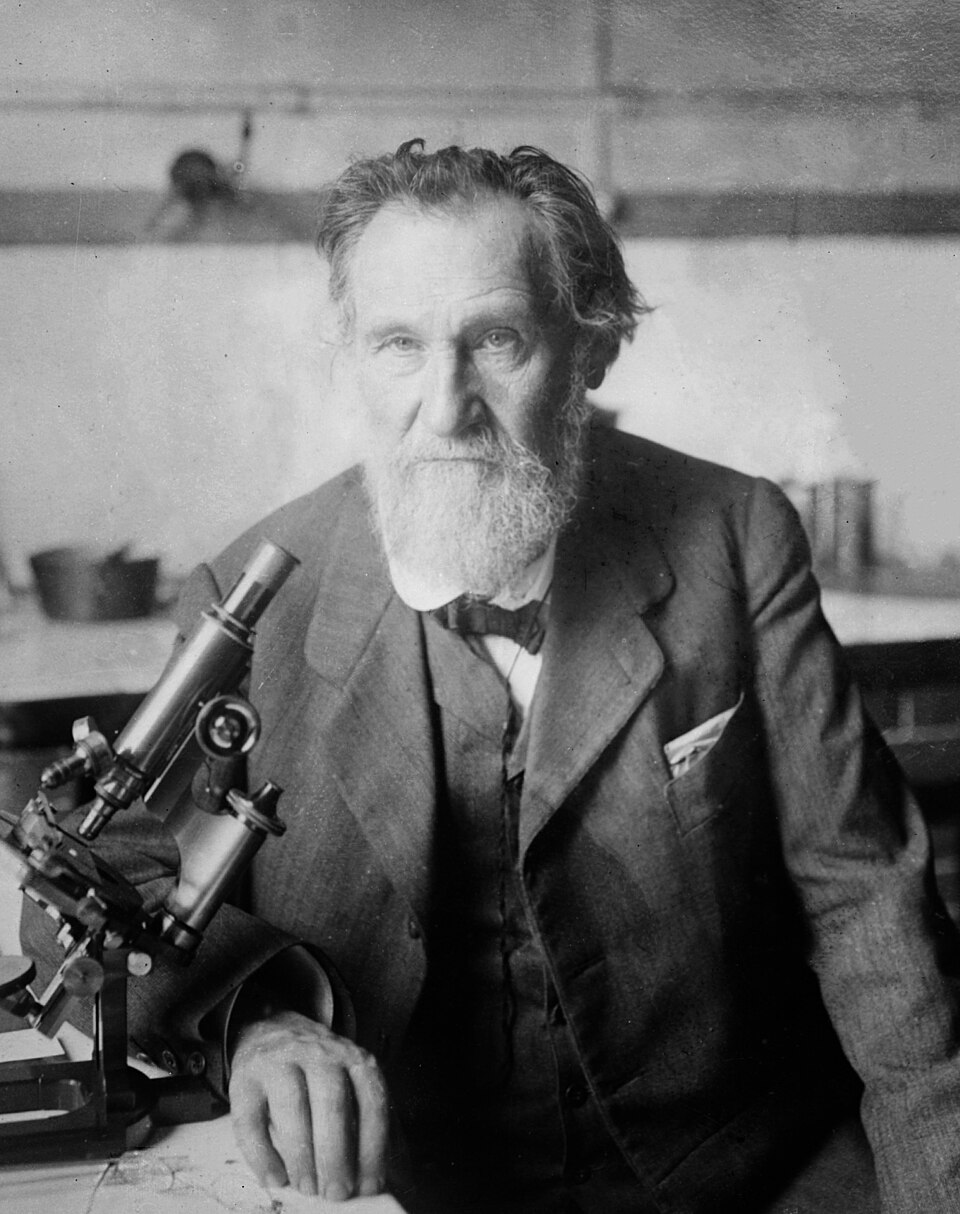
\includegraphics[width=0.30\linewidth]{images/book5/metchnikoff.jpg}\hspace{0.04\linewidth}
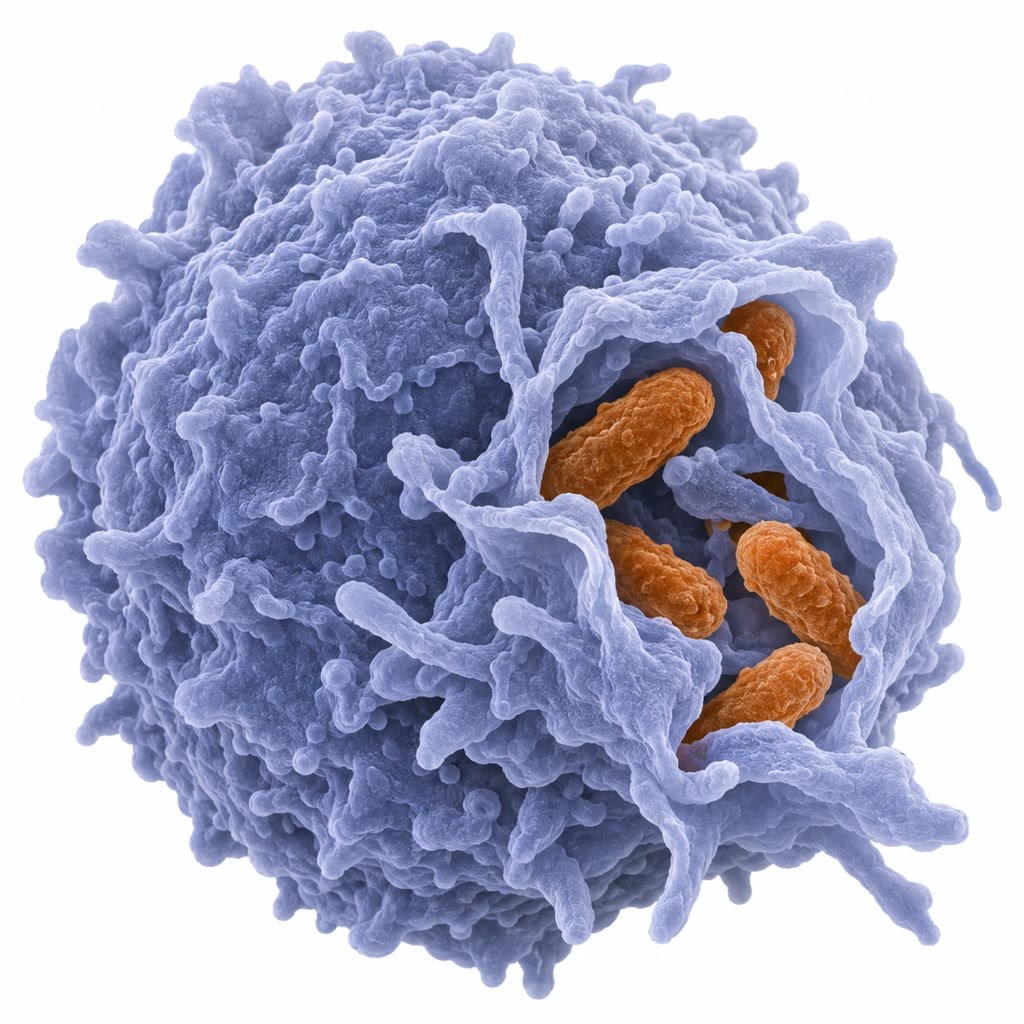
\includegraphics[width=0.30\linewidth]{images/book5/ai/b5-15-neutrophil-phagocytosis.jpg}\hspace{0.04\linewidth}
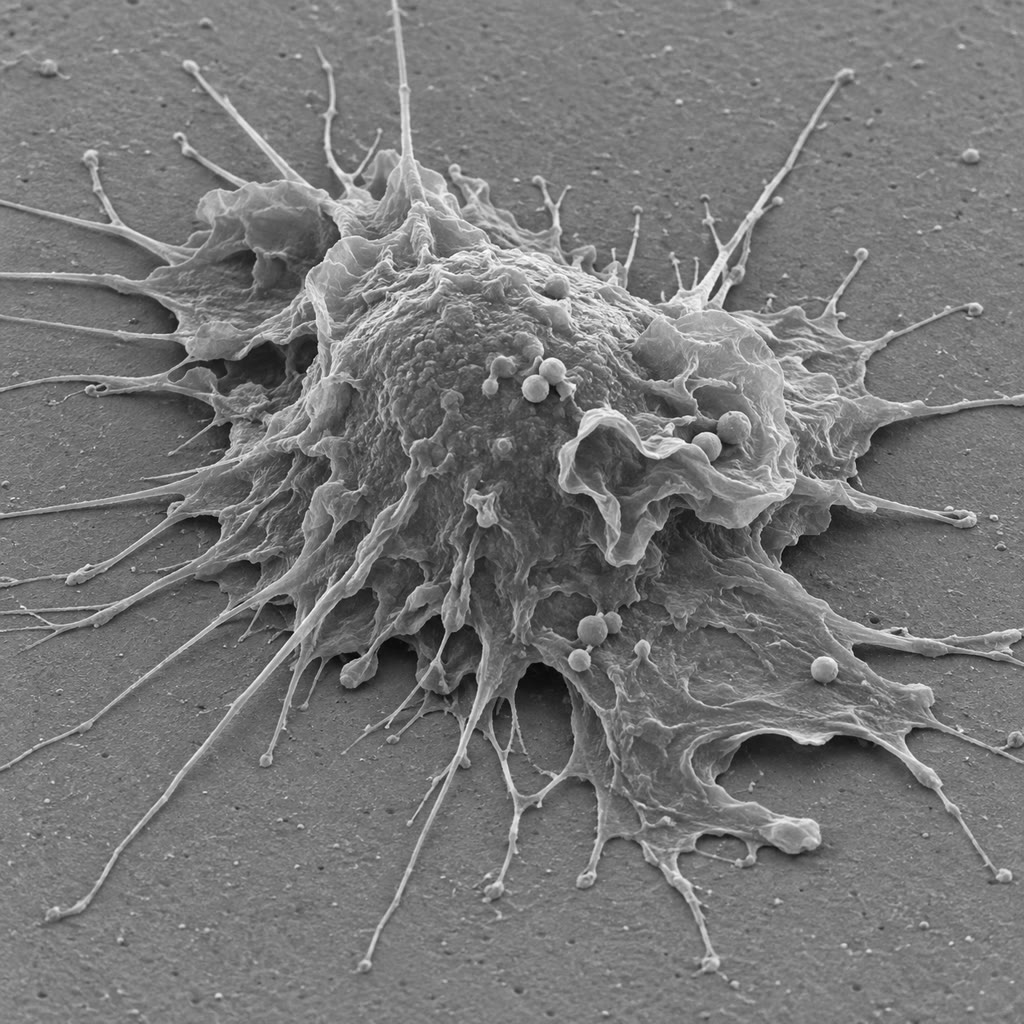
\includegraphics[width=0.30\linewidth]{images/book5/ai/b5-15-macrophage.jpg}

{\small 梅契尼科夫，观察到吞噬细胞聚集于
海星幼虫的刺周围，并开创了细胞免疫学（美国国会图书馆
，公有领域）。中图：正在吞噬细菌的\omterm{def:b3:innate-immunity:innate}{中性粒细胞}。
右图：\omterm{def:b3:innate-immunity:innate}{巨噬细胞}在表面上铺展其皱褶的膜。}
\end{omfigure}

\section{识别入侵者}

\begin{definition}[模式识别]\label{def:b3:innate-immunity:prr}
\index{模式识别受体}\index{病原体相关分子模式}\index{Toll 样受体}\index{损伤相关分子模式}\index{炎症小体}
\omterm{def:b3:innate-immunity:innate}{先天免疫}细胞识别\emph{病原体相关分子模式}
（PAMPs）：一类分子，为整类微生物所共有，对其生存必不可少，
而宿主中不存在——如\omterm{def:b3:bacteriology:envelope}{革兰氏阴性}菌细胞壁的\omterm{def:b3:bacteriology:envelope}{脂多糖}、
\omterm{def:b3:bacteriology:envelope}{革兰氏阳性}菌的\omterm{def:b3:bacteriology:envelope}{肽聚糖}与脂磷壁酸、
鞭毛蛋白、真菌的 $\beta$-葡聚糖、双链 RNA、无
5$'$ 帽的 RNA、未甲基化的 \omterm{def:b3:chromatin-epigenetics:methylation}{CpG} DNA、胞质中的 DNA。
受体即\emph{模式识别受体}（PRRs），共数十种，
每种由一个基因编码：\emph{Toll 样受体}（TLRs）位于
细胞表面及\omterm{def:b3:membrane-traffic:endocytosis}{内体}中（TLR4 识别\omterm{def:b3:bacteriology:envelope}{脂多糖}，TLR5 识别
鞭毛蛋白，TLR3 识别双链 RNA，TLR9 识别 \omterm{def:b3:chromatin-epigenetics:methylation}{CpG} DNA）；
胞质中的 NOD 蛋白识别\omterm{def:b3:bacteriology:envelope}{肽聚糖}片段，RIG-I 识别\omterm{def:b3:virology:virus}{病毒}
RNA，cGAS--STING 识别胞质 DNA；C 型凝集素识别真菌糖类。
同样的受体，或同族的其他受体，还能识别
由受损细胞释放的\emph{\omterm{def:b3:dna-repair:lesions}{损伤}相关分子模式}（DAMPs）
如 ATP、尿酸、核蛋白 HMGB1 与线粒体 DNA——
从而使无菌性\omterm{def:b3:dna-repair:lesions}{损伤}也会引发\omterm{def:b3:innate-immunity:inflammation}{炎症}。
结合后激活转录因子 NF-$\kappa$B 与\omterm{prop:b3:virology:pathogenesis}{干扰素}
调节因子，它们在一小时之内开启\omterm{def:b3:innate-immunity:inflammation}{细胞因子}、\omterm{def:b3:innate-immunity:inflammation}{趋化因子}、黏附分子与
抗菌基因；一部分胞质传感器
\omterm{def:b3:genomics:assembly}{组装}为\emph{\omterm{def:b3:innate-immunity:inflammation}{炎症}小体}，这是一个平台，可激活 caspase-1
使白细胞介素-1$\beta$ 切割为其活性形式，并引发\omterm{def:b3:innate-immunity:inflammation}{炎症}性死亡，
即\omterm{def:b3:cell-cycle-apoptosis:other}{细胞焦亡}（见\cref{ch:b3:cell-cycle-apoptosis}）。
\end{definition}

\begin{proof}[证据]
贾内韦于 1989 年提出，适应性免疫系统不仅对抗原作出应答，
还需要已识别微生物模式的先天受体发出的信号，
这正是\omterm{def:b3:virology:drugs}{疫苗}为何需要\omterm{prop:b3:innate-immunity:bridge}{佐剂}，此即“免疫学家的一个肮脏小秘密”。
霍夫曼
（1996 年）发现，缺失受体 Toll 的 \emph{Drosophila}，
该受体因其在胚胎模式形成中的作用而著称，无法启动抗真菌
应答，身上长满霉菌而死；博伊特勒（1998 年）定位了
一个小鼠品系对\omterm{def:b3:bacteriology:envelope}{脂多糖}的抗性，该品系能耐受
对其他小鼠致死剂量的内毒素，却无法清除\omterm{def:b3:bacteriology:envelope}{革兰氏阴性}菌
感染，这一抗性源于哺乳动物同源基因 TLR4 的突变。该受体
即内毒素的受体，苦寻五十年，原来竟是一个 Toll。
\end{proof}

\begin{omfigure}
\begin{tikzpicture}[every node/.style={font=\scriptsize}, >=stealth]
  % membrane
  \draw[very thick, omDef] (0,3.0) -- (11.5,3.0); \draw[very thick, omDef] (0,2.7) -- (11.5,2.7);
  \node[above] at (0.5,3.05) {膜外}; \node[below] at (0.5,2.65) {胞质};
  % TLR4 with LPS
  \draw[thick, fill=omProp!35] (2.2,2.4) rectangle (2.6,3.9); \draw[thick, fill=omProp!35] (2.9,2.4) rectangle (3.3,3.9);
  \fill[omThm] (2.75,4.1) circle (0.14); \node[above] at (2.75,4.25) {LPS（一种 PAMP）};
  \node[right, align=left] at (3.4,3.5) {TLR4 二聚体 \\与 MD2 结合};
  % signalling
  \node[draw, thick, rounded corners, fill=omDef!20] (myd) at (2.75,1.7) {MyD88、激酶};
  \node[draw, thick, rounded corners, fill=omDef!20] (nfkb) at (2.75,0.6) {NF-$\kappa$B 释放};
  \node[draw, thick, rounded corners, fill=omMeth!25, align=center] (genes) at (2.75,-0.8) {TNF、IL-1$\beta$、IL-6、IL-8；\\黏附分子；iNOS};
  \draw[->, thick] (2.75,2.4) -- (myd); \draw[->, thick] (myd) -- (nfkb); \draw[->, thick] (nfkb) -- (genes);
  \node[right, font=\tiny] at (3.3,1.2) {一小时之内};
  % cytosolic sensors
  \node[draw, thick, rounded corners, fill=omProp!25, align=center] (rig) at (6.9,1.9) {RIG-I：病毒 RNA\\cGAS--STING：胞质 DNA};
  \node[draw, thick, rounded corners, fill=omMeth!25] (ifn) at (6.9,-0.2) {I 型干扰素};
  \draw[->, thick] (rig) -- node[midway, right] {IRF3, IRF7} (ifn);
  \node[draw, thick, rounded corners, fill=omThm!20, align=center] (nlrp) at (10.9,1.9) {NLRP3 炎症小体：\\晶体、ATP、孔};
  \node[draw, thick, rounded corners, fill=omMeth!25, align=center] (il1) at (10.9,-0.8) {caspase-1：IL-1$\beta$\\释放；细胞焦亡};
  \draw[->, thick] (nlrp) -- (il1);
  \draw[->, thick, dashed] (genes.south) -- ++(0,-0.5) -| (il1.south) node[pos=0.25, below, font=\tiny] {pro-IL-1$\beta$ 由 TLR 通路提供};
\end{tikzpicture}

{\small 模式识别的三条途径。表面的 Toll 样受体结合\omterm{def:b3:bacteriology:envelope}{脂多糖}后，
经 NF-$\kappa$B 诱导炎性\omterm{def:b3:innate-immunity:inflammation}{细胞因子}；胞质中识别\omterm{def:b3:virology:virus}{病毒}核酸的
传感器诱导\omterm{prop:b3:virology:pathogenesis}{干扰素}；\omterm{def:b3:innate-immunity:prr}{炎症小体}将储存的白细胞介素-1 前体
转化为
有活性的\omterm{def:b3:innate-immunity:inflammation}{细胞因子}。}
\end{omfigure}

\begin{definition}[补体]\label{def:b3:innate-immunity:complement}
\index{补体}\index{C3 转化酶}\index{调理作用}\index{膜攻击复合物}\index{过敏毒素}
\emph{补体}是一组约三十种血浆蛋白组成的系统，
占血清球蛋白的 \qty{10}{\%}，通过级联的蛋白水解激活来标记并清除微生物。
三条途径汇聚于中央蛋白 C3 的裂解：\emph{经典}途径
由 C1q 结合表面抗体启动（或由 C 反应蛋白、凋亡细胞启动）；
\emph{凝集素}途径由甘露糖结合凝集素识别微生物糖类启动；
\emph{旁路}途径中，C3 以低速率自发水解，
生成的 C3b 附着于其所遇到的任何表面。每条途径都形成一个
\emph{C3 转化酶}，即能裂解更多 C3 的酶；
它沉积于表面的 C3b 又共价结合，
进而形成更多转化酶，构成放大环路，
使一个细菌在几分钟内被数百万个 C3b 包被。
C3b 是一种\emph{调理素}：吞噬细胞带有其受体，
能吞噬被它包被的物质。小片段 C3a 与 C5a 是
\emph{过敏毒素}，可使血管扩张、吸引\omterm{def:b3:innate-immunity:innate}{中性粒细胞}
并激活肥大细胞。C5b 装配 C6--C9，
形成\emph{膜攻击复合物}，即直径 \qty{10}{nm} 的孔道，
可裂解\omterm{def:b3:bacteriology:envelope}{革兰氏阴性}菌及\omterm{def:b3:virology:virus}{包膜}\omterm{def:b3:virology:virus}{病毒}。宿主细胞
因带有调节因子（因子 H、CD55、CD59）而得以幸免，
这些因子在其自身表面拆解转化酶并阻断孔道；
微生物缺乏此类调节因子，
因而被环路消耗。
\end{definition}

\begin{theorem}[补体环路作为动力学判别机制]\label{thm:b3:innate-immunity:complement}
\index{补体!放大环路}
设 $B(t)$ 为沉积于表面的 C3b 分子数。C3b
以来自 C3 自发缓慢水解的较小恒定速率 $k_{0}$ 沉积，
每个已沉积的 C3b 形成转化酶，进而
以每个 C3b 每秒 $a$ 的速率再沉积更多 C3b；同时，调节因子（宿主）与衰减
每个 C3b 每秒 $d$ 的速率消除转化酶活性：
\[
\frac{\mathrm{d}B}{\mathrm{d}t} = k_{0} + (a - d)\,B .
\]
在满足 $a > d$ 的表面上——即无调节因子的微生物——
$B(t) = \bigl[k_{0}/(a-d)\bigr]\bigl(e^{(a-d)t} - 1\bigr)$ 随时间
呈指数增长，时间常数为 $1/(a - d)$；在宿主表面上，
$d > a$ 时，$B$ 趋于很小的稳态值 $k_{0}/(d - a)$。
同样的分子，同样的浓度，在一个细菌上几分钟内
即可沉积 100 万个 C3b，而在旁边的细胞上只沉积几十个：
自身与非自身的区分并非由识别完成，而是由
$a - d$ 的符号决定。
\end{theorem}
\begin{proof}
方程为线性常系数方程。当 $a \ne d$ 时，
不动点为 $B^{*} = -k_{0}/(a-d)$；记 $B = B^{*} + u$，
则 $\mathrm{d}u/\mathrm{d}t = (a-d)u$，故 $u = u_{0}e^{(a-d)t}$，
由 $B(0) = 0$ 得 $B(t) = \bigl[k_{0}/(a-d)\bigr](e^{(a-d)t} - 1)$。当 $a > d$ 时，
该式无界增长（直至 C3 或表面耗尽）；当 $a < d$ 时，
指数衰减，$B \to k_{0}/(d-a) > 0$。取 $k_{0} = 1$ 每秒，
在细菌上 $a - d = \qty{0.1}{s^{-1}}$，$B(\qty{2}{min})
= 10(e^{12} - 1) \approx 1.6\times 10^{6}$；在宿主细胞上 $d - a =
\qty{0.1}{s^{-1}}$，$B^{*} = 10$。
\end{proof}

\begin{omfigure}
\begin{tikzpicture}
\begin{axis}[
  width=0.66\linewidth, height=5.6cm,
  axis x line=bottom, axis y line=left,
  xmin=0, xmax=150, ymin=1, ymax=1e7, ymode=log,
  xlabel={秒}, ylabel={已沉积的 C3b},
  xlabel style={font=\small, at={(axis description cs:0.5,-0.12)}, anchor=north}, ylabel style={font=\small},
  tick label style={font=\small}, xtick={0,30,60,90,120,150},
  clip=false,
]
\addplot[very thick, omThm, domain=1:150, samples=80] {10*(exp(0.1*x)-1)};
\addplot[very thick, omDef, domain=1:150, samples=80] {10*(1-exp(-0.1*x))};
\node[font=\scriptsize, omThm, anchor=east] at (axis cs:100,2e5) {微生物：$a > d$，指数增长};
\node[font=\scriptsize, omDef, anchor=south west] at (axis cs:60,14) {宿主细胞：$d > a$，饱和于 $k_{0}/(d-a)$};
\end{axis}
\end{tikzpicture}

{\small 两个表面上的\omterm{def:b3:innate-immunity:complement}{补体}环路，取 $k_{0} = 1$ 每秒，
$|a - d| = \qty{0.1}{s^{-1}}$：在缺乏调节因子的微生物上，C3b
呈指数增长，两分钟内达到 100 万；在具有调节因子的宿主细胞上，
则趋于平稳，稳定在 10。}
\end{omfigure}

\begin{omfigure}
\begin{tikzpicture}[every node/.style={font=\scriptsize}, >=stealth]
  \node[draw, thick, rounded corners, fill=omDef!20, align=center] (cl) at (-4.2,3.0) {经典途径：\\抗体上的 C1q\\或 C 反应蛋白};
  \node[draw, thick, rounded corners, fill=omDef!20, align=center] (le) at (0,3.0) {凝集素途径：\\甘露糖结合凝集素 \\识别微生物糖类};
  \node[draw, thick, rounded corners, fill=omDef!20, align=center] (al) at (4.2,3.0) {旁路途径：\\C3 自发缓慢水解，\\C3b 附着于任何表面};
  \node[draw, thick, rounded corners, fill=omProp!35, minimum width=3cm] (conv) at (0,1.2) {C3 转化酶};
  \node[draw, thick, rounded corners, fill=omThm!25, align=center] (c3b) at (0,-0.4) {C3 $\to$ C3b（位于表面）$+$ C3a};
  \draw[->, thick] (cl) -- (conv); \draw[->, thick] (le) -- (conv); \draw[->, thick] (al) -- (conv);
  \draw[->, thick] (conv) -- (c3b);
  \draw[->, very thick, omThm] (c3b.east) .. controls (3.2,-0.4) and (3.2,1.2) .. (conv.east) node[pos=0.5, right, align=left] {放大环路：\\C3b 形成更多转化酶};
  \node[draw, thick, rounded corners, fill=omMeth!25, align=center] (ops) at (-4.4,-2.2) {调理作用：\\吞噬细胞吞噬 \\被 C3b 包被的物质};
  \node[draw, thick, rounded corners, fill=omMeth!25, align=center] (ana) at (0,-2.2) {C3a、C5a：\\血管扩张，中性粒细胞 \\与肥大细胞被募集};
  \node[draw, thick, rounded corners, fill=omMeth!25, align=center] (mac) at (4.4,-2.2) {C5b--C9：\\膜攻击复合物，\\裂解};
  \draw[->, thick] (c3b) -- (ops); \draw[->, thick] (c3b) -- (ana); \draw[->, thick] (c3b) -- (mac);
  \node[draw, thick, rounded corners, fill=gray!15, align=center] (reg) at (-4.4,1.2) {宿主调节因子：\\因子 H、CD55、CD59};
  \draw[-|, thick, gray!60!black] (reg) -- (conv);
\end{tikzpicture}

{\small \omterm{def:b3:innate-immunity:complement}{补体}。三条途径各自形成一个 C3 转化酶；其沉积的 C3b
又形成更多转化酶（即定理中的环路），沉积的 C3b 起\omterm{def:b3:innate-immunity:complement}{调理作用}，
片段引发\omterm{def:b3:innate-immunity:inflammation}{炎症}，末端复合物使靶细胞裂解。宿主
细胞带有调节因子，可切断环路（并与 CD59 一道阻断孔道），
这些因子位于其自身膜上。}
\end{omfigure}

\section{炎症}

\begin{definition}[急性炎症]\label{def:b3:innate-immunity:inflammation}
\index{炎症}\index{细胞因子}\index{趋化因子}\index{渗出}\index{选择素}\index{整合素}
\emph{炎症}是有血管组织对\omterm{def:b3:dna-repair:lesions}{损伤}或
感染所作的反应，由\emph{细胞因子}——免疫细胞的小型信号蛋白，
此处主要指活化\omterm{def:b3:innate-immunity:innate}{巨噬细胞}分泌的 TNF、白细胞介素-1 和白细胞介素-6——
以及\emph{趋化因子}（引导迁移的细胞因子）共同调控。
其各步骤可解释塞尔苏斯所描述的征象。组胺来自肥大细胞，
一氧化氮和前列腺素使小动脉扩张，产生\emph{发红}和\emph{局部\omterm{prop:b3:innate-immunity:systemic}{发热}}。
微静脉内皮收缩并渗漏血浆，
血浆蛋白（\omterm{def:b3:innate-immunity:complement}{补体}、抗体、凝血因子）涌入组织，产生\emph{肿胀}。
缓激肽和前列腺素 E$_{2}$使神经末梢敏感化，产生\emph{疼痛}。
白细胞经\emph{渗出}进入感染部位：
TNF 和白细胞介素-1 使内皮表达\emph{选择素}，
途经的\omterm{def:b3:innate-immunity:innate}{中性粒细胞}借此黏附并滚动；
内皮表面的趋化因子（白细胞介素-8）激活\omterm{def:b3:innate-immunity:innate}{中性粒细胞}的\emph{整合素}，
使其与内皮黏附分子紧密结合而停止；
\omterm{def:b3:innate-immunity:innate}{中性粒细胞}随后挤过内皮细胞之间，
沿趋化因子梯度进入组织——
整个过程仅需数分钟，
每小时可有多达 100 万个细胞进入感染部位。
\end{definition}

\begin{omfigure}
\begin{tikzpicture}[every node/.style={font=\scriptsize}, >=stealth]
  % vessel wall
  \fill[omThm!10] (0,0) rectangle (12,2.3); \node[left, omThm!70!black, anchor=north east] at (12,2.25) {血液，流动 $\rightarrow$};
  \foreach \x in {0,1.5,3,4.5,6,7.5,9,10.5} \draw[thick, fill=omDef!30] (\x,-0.05) rectangle (\x+1.45,0.35);
  \node[right] at (0.1,-0.35) {内皮};
  \fill[omMeth!8] (0,-1.7) rectangle (12,-0.45); \node[right, omMeth!60!black] at (0.1,-1.55) {组织};
  % bacteria and chemokine gradient
  \foreach \p in {(10.6,-1.1),(11.0,-0.9),(11.3,-1.2)} \fill[omProp] \p ellipse (0.14 and 0.07);
  \node[below, omProp] at (11.0,-1.35) {细菌};
  \node[below, font=\tiny] at (8.0,-0.5) {趋化因子梯度 $\rightarrow$};
  % neutrophils in sequence
  \draw[thick, fill=white] (1.2,1.1) circle (0.3); \node[above] at (1.2,1.45) {1. 流动};
  \draw[thick, fill=white] (3.4,0.68) circle (0.3); \node[above] at (3.4,1.05) {2. 沿选择素滚动};
  \draw[omThm, thick] (3.1,0.45) -- (3.05,0.35); \draw[omThm, thick] (3.4,0.38) -- (3.4,0.35); \draw[omThm, thick] (3.7,0.45) -- (3.75,0.35);
  \draw[thick, fill=white] (6.0,0.62) ellipse (0.38 and 0.26); \node[above, align=center] at (6.0,0.95) {3. 牢固黏附 \\（整合素）};
  \draw[thick, fill=white] (8.25,0.18) ellipse (0.2 and 0.42); \node[above, align=center] at (8.4,0.95) {4. 挤压 \\穿过};
  \draw[thick, fill=white] (9.6,-1.0) circle (0.3); \node[left] at (9.25,-1.0) {5. 爬向感染部位};
  \draw[->, thick, gray] (1.5,1.05) -- (3.0,0.8); \draw[->, thick, gray] (3.7,0.68) -- (5.6,0.62); \draw[->, thick, gray] (6.4,0.5) -- (8.0,0.4); \draw[->, thick, gray] (8.3,-0.3) -- (9.3,-0.8);
  % TNF label
  \node[below, align=center, font=\tiny] at (4.0,-1.75) {来自组织巨噬细胞的 TNF 和 IL-1 使内皮表达 \\可捕获中性粒细胞的选择素和黏附分子};
\end{tikzpicture}

{\small \omterm{def:b3:innate-immunity:inflammation}{渗出}。组织\omterm{def:b3:innate-immunity:innate}{巨噬细胞}分泌的\omterm{def:b3:innate-immunity:inflammation}{细胞因子}使
微静脉壁变得具有黏性；途经的\omterm{def:b3:innate-immunity:innate}{中性粒细胞}黏附于\omterm{def:b3:innate-immunity:inflammation}{选择素}上并
滚动，受\omterm{def:b3:innate-immunity:inflammation}{整合素}阻滞而停止，挤过内皮细胞之间，
并沿\omterm{def:b3:innate-immunity:inflammation}{趋化因子}梯度走向细菌。}
\end{omfigure}

\begin{proposition}[发热、急性期反应与消退]\label{prop:b3:innate-immunity:systemic}
\index{发热}\index{急性期反应}\index{C 反应蛋白}\index{炎症消退}
白细胞介素-1、TNF 和白细胞介素-6 也可远距离发挥作用。
在下丘脑，它们诱导前列腺素 E$_{2}$，
后者使体温调定点升高，即\emph{\omterm{prop:b3:innate-immunity:systemic}{发热}}，
可抑制多种细菌，加快免疫细胞自身的反应，
并使每升高一度的代谢约增加\qty{12}{\%}。
在肝脏中，它们诱导\emph{急性期蛋白}——
C 反应蛋白可结合细菌的磷酸胆碱并激活\omterm{def:b3:innate-immunity:complement}{补体}，
两天内升高约一千倍，是临床衡量\omterm{def:b3:innate-immunity:inflammation}{炎症}的指标；
另有纤维蛋白原、甘露糖结合凝集素，
以及铁调素，后者将铁锁定，使需要铁的微生物无从获得。
在骨髓中，它们促使\omterm{def:b3:innate-immunity:innate}{中性粒细胞}释放并加快其生成。
\omterm{def:b3:innate-immunity:inflammation}{炎症}本应终止：刺激被清除后，脂质介质由前列腺素转为
脂氧素和消退素，\omterm{def:b3:innate-immunity:innate}{中性粒细胞}经\omterm{def:b3:cell-cycle-apoptosis:apoptosis}{细胞凋亡}死亡，并被\omterm{def:b3:innate-immunity:innate}{巨噬细胞}吞噬，
\omterm{def:b3:innate-immunity:innate}{巨噬细胞}随之转入修复程序，分泌生长因子和白细胞介素-10，
即\emph{消退}。若刺激持续存在，
例如无法杀灭的结核分枝杆菌、晶体或自身抗原，
反应则转为慢性：\omterm{def:b3:innate-immunity:innate}{巨噬细胞}将病灶包裹为肉芽肿，
成纤维细胞沉积形成瘢痕，
组织最终被自身的防御反应破坏。
\end{proposition}

\begin{example}[脓毒症]\label{ex:b3:innate-immunity:sepsis}
局限于一根木刺周围的\omterm{def:b3:innate-immunity:inflammation}{炎症}是有益的；
同样的反应若遍及全身，则是灾难。
细菌或其\omterm{def:b3:bacteriology:envelope}{脂多糖}大量进入血液时，
各处\omterm{def:b3:innate-immunity:innate}{巨噬细胞}同时释放 TNF 和白细胞介素-1，
所有血管扩张、渗漏，血压骤降，
上万条毛细血管内凝血被激活，消耗凝血因子，
器官因灌注不足而衰竭，即\emph{脓毒性休克}，
它使被\omterm{def:b3:cancer-biology:metastasis}{侵袭}者中四分之一至一半死亡，每年约 1100 万人。
向志愿者注射数微克\omterm{def:b3:bacteriology:envelope}{脂多糖}，两小时内即出现\omterm{prop:b3:innate-immunity:systemic}{发热}、寒战和血压下降；
缺乏 TLR4 的小鼠能耐受百倍致死剂量。
疾病是宿主的反应，
而杀灭细菌的\omterm{def:b3:bacteriology:antibiotics}{抗生素}可能因释放更多内毒素，
使病情在数小时内加重。
\end{example}

\begin{omfigure}
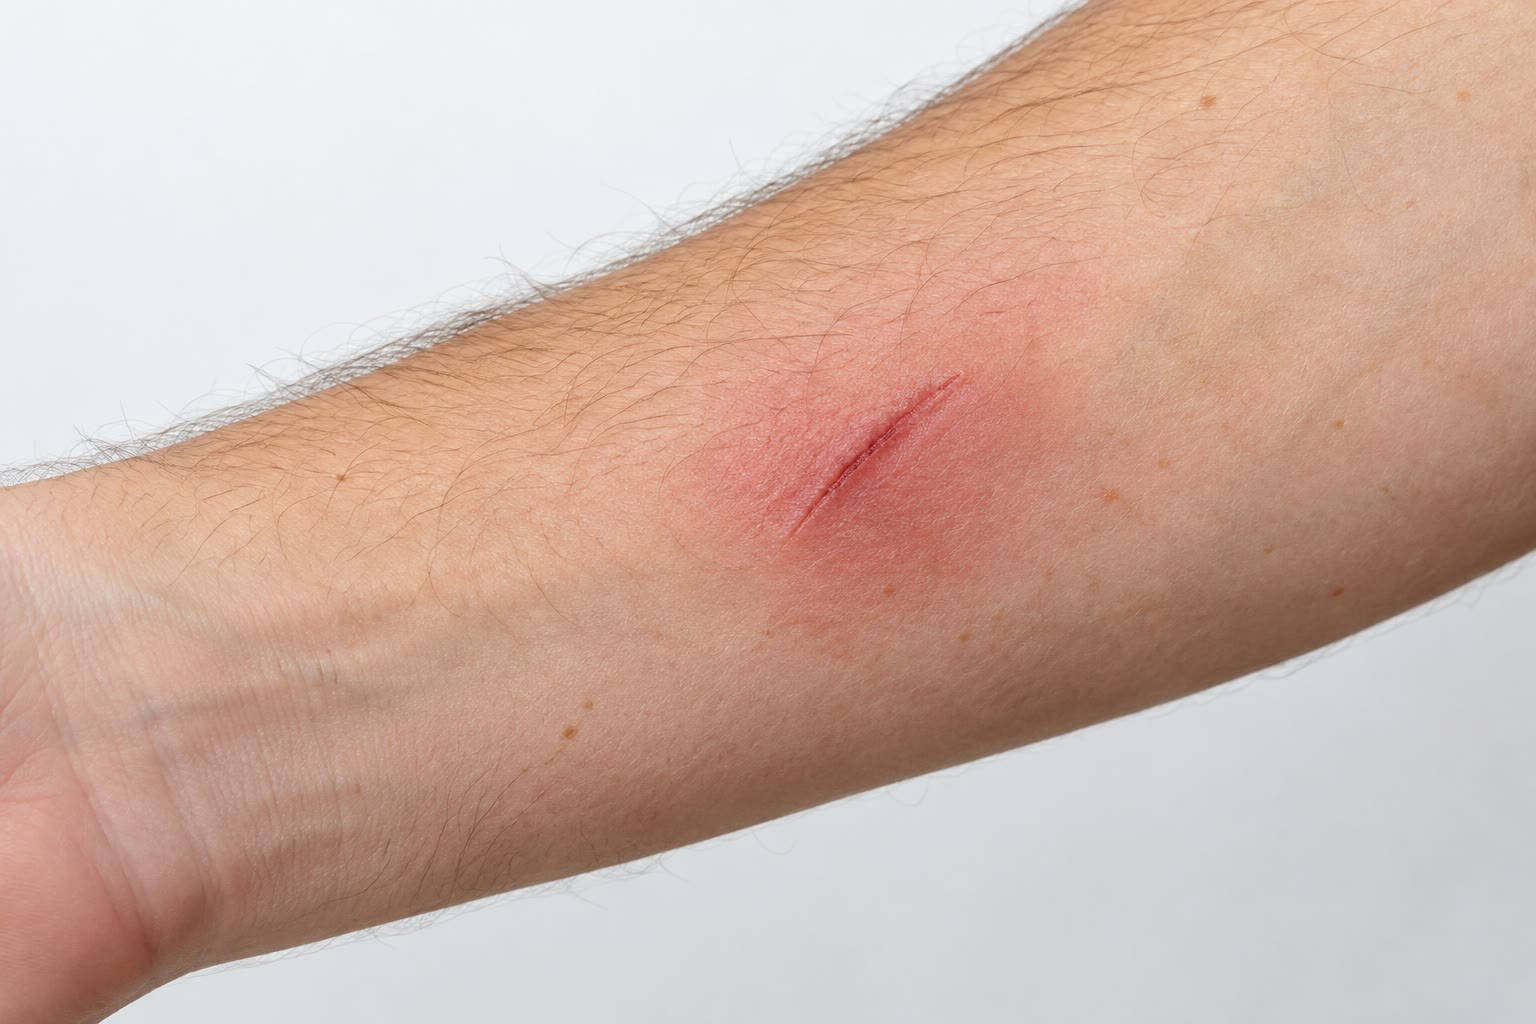
\includegraphics[width=0.52\linewidth]{images/book5/ai/b5-15-inflamed-skin.jpg}

{\small 木刺划伤周围的急性\omterm{def:b3:innate-immunity:inflammation}{炎症}：发红与局部\omterm{prop:b3:innate-immunity:systemic}{发热}，
由扩张血管所致；\omterm{def:b3:innate-immunity:inflammation}{渗出}血浆所致肿胀，
以及使肢体保持不动的疼痛——
这种局部反应若波及全身，即为脓毒性休克。}
\end{omfigure}

\section{杀灭}

\begin{definition}[吞噬作用与呼吸爆发]\label{def:b3:innate-immunity:killing}
\index{吞噬作用}\index{呼吸爆发}\index{NADPH 氧化酶}\index{中性粒细胞胞外诱捕网}
吞噬细胞借调理素的受体结合猎物，调理素包括 C3b
和抗体的恒定区；也可直接通过\omterm{def:b3:innate-immunity:prr}{模式识别受体}结合，
随后将其包入膜中，并闭合形成\emph{吞噬体}，
吞噬体与颗粒和\omterm{def:b3:membrane-traffic:endocytosis}{溶酶体}融合。杀灭作用同时通过多种手段进行。
\emph{呼吸爆发}：酶\emph{NADPH 氧化酶}\omterm{def:b3:genomics:assembly}{组装}于吞噬体膜上，
将电子泵至氧气上生成超氧阴离子，
超氧阴离子转化为过氧化氢，
髓过氧化物酶再与氯离子作用，将其变为次氯酸——即漂白剂，
浓度达毫摩尔级，位于直径仅一微米的小室内。
诱导型一氧化氮合酶产生的一氧化氮，与超氧阴离子结合生成过氧亚硝酸盐。
酸化至 pH~5。溶菌酶、蛋白酶，
使猎物缺铁的乳铁蛋白，以及刺穿猎物的防御素。
若\omterm{def:b3:innate-immunity:innate}{中性粒细胞}无法吞食所遇之物——如真菌菌丝或团块——
便可将自身\omterm{def:b3:chromatin-epigenetics:nucleosome}{染色质}以黏性 DNA 与颗粒蛋白网的形式排出，即\emph{\omterm{def:b3:innate-immunity:innate}{中性粒细胞}
胞外诱捕网}，并随之死亡。遗传上 NADPH 氧化酶有缺陷的患儿
（慢性肉芽肿病）反复出现由细菌和真菌引起的脓肿与肉芽肿，
这些病原体普通吞噬细胞本可轻易杀灭：
呼吸爆发并非可有可无。
\end{definition}

\begin{definition}[自然杀伤细胞与干扰素]\label{def:b3:innate-immunity:nk-ifn}
\index{自然杀伤细胞!缺失自我}\index{干扰素!I 型}\index{抗病毒状态}
\omterm{def:b3:virology:virus}{病毒}藏身于细胞内，
\omterm{def:b3:innate-immunity:complement}{补体}与吞噬细胞都够不着它们。\emph{\omterm{def:b3:innate-immunity:innate}{自然杀伤细胞}}巡查那些
已停止呈递 MHC~I 类分子的细胞——
即“缺失自我”的细胞，其内的\omterm{def:b3:virology:virus}{病毒}或\omterm{def:b3:cancer-biology:hallmarks}{肿瘤}已关闭抗原呈递，
以逃避 T~细胞（\cref{ch:b3:adaptive-immunity}）——并巡查
感染细胞与转化细胞表面出现的应激蛋白；
MHC~I 的抑制性受体与应激配体的激活性受体信号相加，
哪一侧占优，该细胞便在数分钟内被杀伤：
穿孔素与颗粒酶注入其中，诱导其凋亡。
\emph{I~型\omterm{prop:b3:virology:pathogenesis}{干扰素}}（$\alpha$ 与 $\beta$）由任何一个 RIG-I 或 cGAS 检测到\omterm{def:b3:virology:virus}{病毒}核酸的细胞产生；
分泌后，它们与邻近细胞的受体结合，
经 JAK--STAT 通路诱导数百个基因表达，使这些细胞进入
\emph{抗\omterm{def:b3:virology:virus}{病毒}状态}：遇到双链 RNA 时，一种激酶关闭翻译；
一种核酸酶降解 RNA；若干蛋白阻止\omterm{def:b3:virology:virus}{病毒}侵入与\omterm{def:b3:genomics:assembly}{组装}；
此外，MHC~I 分子增多，向 T~细胞展示细胞内的情况。
产生\omterm{prop:b3:virology:pathogenesis}{干扰素}的细胞可能就此死亡，
而其邻居已得到预警。
\omterm{prop:b3:virology:pathogenesis}{干扰素}由 Isaacs 与 Lindenmann 于 1957 年发现，
是\omterm{def:b3:virology:virus}{病毒}感染细胞的培养基中使新鲜细胞产生抗性的因子，
也正因如此，一个已被某种\omterm{def:b3:virology:virus}{病毒}感染的细胞
能抵抗第二种\omterm{def:b3:virology:virus}{病毒}。
\end{definition}

\begin{method}[炎症与吞噬细胞功能的测定]\label{met:b3:innate-immunity:tests}
\index{C 反应蛋白!测定}\index{硝基蓝四唑试验}
床旁可做以下检测：(1) 血清中的\emph{C 反应蛋白}，
以免疫测定法测定——静息时低于 \qty{5}{mg/L}，
\omterm{def:b3:virology:virus}{病毒}感染时为数十，细菌性脓毒症时可达数百，
有效治疗后数日内下降；
(2) \omterm{def:b3:innate-immunity:innate}{中性粒细胞}计数，细菌感染时升高，
未成熟形式较早自骨髓释放；
(3) 红细胞沉降率，是纤维蛋白原的一种缓慢替代指标。
对吞噬细胞：(4) \emph{硝基蓝四唑}或二氢罗丹明检测，
体外受刺激的\omterm{def:b3:innate-immunity:innate}{中性粒细胞}，若其 NADPH 氧化酶正常，则可还原染料——
一个上午即可诊断慢性肉芽肿病；
(5) 趋化试验，计数穿过滤膜、向\omterm{def:b3:innate-immunity:inflammation}{趋化因子}迁移的细胞。
\end{method}

\section{从先天免疫到适应性免疫，及跨越生命的历程}

\begin{proposition}[树突状细胞的抉择]\label{prop:b3:innate-immunity:bridge}
\index{树突状细胞!成熟}\index{共刺激}\index{佐剂}
适应性免疫并非自行启动。
组织中的\emph{\omterm{def:b3:innate-immunity:innate}{树突状细胞}}吞食所遇之物；
若其\omterm{def:b3:innate-immunity:prr}{模式识别受体}被触发——
无论由微生物还是由\omterm{def:b3:dna-repair:lesions}{损伤}所致——它便成熟：停止吞食，
经淋巴管迁至引流淋巴结，
在 MHC 分子上展示所吞食物的肽段，
并表达\emph{共刺激}分子（B7）与\omterm{def:b3:innate-immunity:inflammation}{细胞因子}，
告知识别该肽段的 T~细胞是否应答、如何应答（\cref{ch:b3:adaptive-immunity}）。
若 T~细胞在缺乏共刺激的\omterm{def:b3:innate-immunity:innate}{树突状细胞}上见到其肽段，
则会被关闭。
由此，先天识别决定抗原是否值得应答；
\omterm{def:b3:innate-immunity:innate}{树突状细胞}所产生的\omterm{def:b3:innate-immunity:inflammation}{细胞因子}——由哪些\omterm{def:b3:innate-immunity:prr}{模式识别受体}被激活所决定——
则决定应答针对\omterm{def:b3:virology:virus}{病毒}、细菌还是蠕虫。
\emph{\omterm{prop:b3:innate-immunity:bridge}{佐剂}}是添加到\omterm{def:b3:virology:drugs}{疫苗}中、以提供此信号的\omterm{def:b3:innate-immunity:prr}{模式识别受体}配体；
现代\omterm{def:b3:virology:drugs}{疫苗}中的明矾与脂质纳米颗粒，正是通过触发该信号而起作用。
\end{proposition}

\begin{remark}[处处皆有的先天免疫及其记忆]\label{rem:b3:innate-immunity:everywhere}
每一种多细胞生物都具有\omterm{def:b3:innate-immunity:innate}{先天免疫}，而植物、真菌与无脊椎动物则只有\omterm{def:b3:innate-immunity:innate}{先天免疫}。
植物以受体激酶识别鞭毛蛋白与几丁质，并启动两级应答（\cref{ch:b3:plant-molecular-physiology}）；
昆虫具有 Toll 与抗菌肽；
甚至细菌也有\omterm{def:b3:genetic-engineering:tools}{限制酶}与 \omterm{def:b3:genetic-engineering:crispr}{CRISPR}（\cref{ch:b3:genetic-engineering}）。
\omterm{def:b3:innate-immunity:innate}{先天免疫}没有记忆的教条已有所松动：
接触过 $\beta$-葡聚糖或卡介苗的单核细胞，
会发生表观遗传\omterm{def:b3:chromatin-epigenetics:epigenetics}{重编程}（\cref{ch:b3:chromatin-epigenetics}），
在数月内对无关微生物的应答更为强烈——
即\emph{训练免疫}，
这也解释了为何卡介苗能降低婴儿因结核以外感染而导致的死亡率。
而该系统的过度活动是我们这个时代的一种疾病：
由尿酸晶体引发的无菌性\omterm{def:b3:innate-immunity:inflammation}{炎症}（痛风）、
动脉壁中的胆固醇晶体（动脉粥样硬化）、
脑中的\omterm{def:b3:structural-biology:amyloid}{淀粉样蛋白}，
以及肥胖和老年期的低度\omterm{def:b3:innate-immunity:inflammation}{炎症}。
\end{remark}

\section{练习}

\begin{exercise}[$\star$]\label{exo:b3:innate-immunity:1}
列出\omterm{def:b3:innate-immunity:innate}{先天免疫}的四种\omterm{def:b3:innate-immunity:innate}{屏障}与五类细胞，
并各说明一项功能。
\end{exercise}

\begin{exercise}[$\star$]\label{exo:b3:innate-immunity:2}
何种分子才能成为良好的\omterm{def:b3:innate-immunity:prr}{病原体相关分子模式}？
举出三例，并说明每例对应的受体。
\end{exercise}

\begin{exercise}[$\star$]\label{exo:b3:innate-immunity:3}
以一种介质及一项血管或神经变化，
解释 Celsus 的四个体征中的每一个。
\end{exercise}

\begin{exercise}[$\star$]\label{exo:b3:innate-immunity:4}
写出三条\omterm{def:b3:innate-immunity:complement}{补体}途径，
说明各自由何启动，以及 C3 裂解的三种结果。
\end{exercise}

\begin{exercise}[$\star\star$]\label{exo:b3:innate-immunity:5}
在\omterm{def:b3:innate-immunity:complement}{补体}模型中，设 $k_{0} = 2$ 每秒，$a =
\qty{0.15}{s^{-1}}$，$d = \qty{0.05}{s^{-1}}$，对微生物而言，经过 \qty{60}{s} 后沉积了多少个 C3b？
经过 \qty{90}{s} 后又为多少？若宿主细胞上 $a = 0.05$，$d = 0.15$，
其稳态为何？
\end{exercise}

\begin{exercise}[$\star\star$]\label{exo:b3:innate-immunity:6}
排列\omterm{def:b3:innate-immunity:inflammation}{渗出}过程的各个事件，指出每一步涉及的分子类别，
并预测一名\omterm{def:b3:innate-immunity:innate}{中性粒细胞}缺乏患儿的表型——
该患儿\omterm{def:b3:innate-immunity:innate}{中性粒细胞}缺乏 $\beta_{2}$ \omterm{def:b3:innate-immunity:inflammation}{整合素}（白细胞黏附缺陷）。
\end{exercise}

\begin{exercise}[$\star\star$]\label{exo:b3:innate-immunity:7}
患者的\omterm{def:b3:innate-immunity:innate}{中性粒细胞}未能通过二氢罗丹明试验。诊断为何？
缺失的是哪一步反应，以及预期会出现哪些
感染？为何会形成肉芽肿？
\end{exercise}

\begin{exercise}[$\star\star$]\label{exo:b3:innate-immunity:8}
说明“缺失自身”识别，并预测\omterm{def:b3:cancer-biology:hallmarks}{肿瘤}
细胞分别 (a) 为逃避 T 细胞而丢失 MHC~I，(b) 保留 MHC~I 但
展示应激配体。
\end{exercise}

\begin{exercise}[$\star\star$]\label{exo:b3:innate-immunity:9}
为何纯蛋白质\omterm{def:b3:virology:drugs}{疫苗}诱导的免疫很弱，
\omterm{prop:b3:innate-immunity:bridge}{佐剂}又增加了什么？请结合詹韦的论证加以说明。
\end{exercise}

\begin{exercise}[$\star\star\star$]\label{exo:b3:innate-immunity:10}
\omterm{prop:b3:innate-immunity:systemic}{发热}每升高一度，静息代谢额外消耗 \qty{12}{\%}，并使
细菌的倍增时间从 \qty{37}{\celsius} 时的 \qty{30}{min}
延长至 \qty{40}{\celsius} 时的 \qty{45}{min}。在感染一天内，计算
在有\omterm{prop:b3:innate-immunity:systemic}{发热}与无\omterm{prop:b3:innate-immunity:systemic}{发热}两种情况下，由 $10^{4}$ 个细菌出发的细菌数量（忽略杀伤），
以及一名 \qty{8}{MJ/d} 的人多消耗的能量。
\omterm{prop:b3:innate-immunity:systemic}{发热}是否值得？答案取决于什么？
\end{exercise}

\begin{exercise}[$\star\star\star$]\label{exo:b3:innate-immunity:11}
有些细菌在表面结合因子 H，另一些切割 C3b 或脱落荚膜。
利用\cref{thm:b3:innate-immunity:complement}，
将每种情况解释为 $a$ 或 $d$ 的改变，并说明哪一种
对微生物而言是最经济的防御方式。
\end{exercise}

\begin{exercise}[$\star\star\star$]\label{exo:b3:innate-immunity:12}
结合本章机制论证，为何同一反应在刺伤处是适应性的，
而在血流中却是致命的，并说明为何阻断 TNF 的药物
有助于治疗类风湿性关节炎，却会增加
结核病的风险？
\end{exercise}

\section{问题：一根木刺}

\begin{problem}[{周末问题——皮下一万个细菌
与赶来迎战的中性粒细胞竞速，经回路运算被补体包覆，
以代谢代价与发热抗争，
在血流中演变为休克的生理过程，
并以六小时后残余的细菌数、各细菌上的 C3b
及一天发热的代价作结。}]
\label{pb:b3:innate-immunity:1}
数据：接种 $10^{4}$ 个细菌，每 \qty{40}{min} 倍增一次；
\omterm{def:b3:innate-immunity:innate}{中性粒细胞}自 \qty{1}{h} 起到达，速率为每小时 $2\times 10^{4}$ 个，每个
可杀死 $20$ 个细菌，随后死亡。\omterm{def:b3:innate-immunity:complement}{补体}：每个细菌每秒 $k_{0} = 1$，
细菌上 $a - d = \qty{0.08}{s^{-1}}$，宿主细胞上 $d - a =
\qty{0.1}{s^{-1}}$；一个细菌表面最多可容纳
$2\times 10^{6}$ 个 C3b。\omterm{prop:b3:innate-immunity:systemic}{发热} $+\qty{2}{\celsius}$ 额外消耗 \qty{24}{\%}
的 \qty{8}{MJ/d} 代谢量，并使细菌
倍增时间延长至 \qty{60}{min}。败血症：$10^{9}$ 个细菌位于 \qty{5}{L} 血液中，
每个细菌含 $3\times 10^{6}$ 个\omterm{def:b3:bacteriology:envelope}{脂多糖}分子；TLR4
信号传导在\omterm{def:b3:bacteriology:envelope}{脂多糖}浓度达 $10^{-9}$ mol/L 时饱和。

\medskip
\noindent\textbf{第一部分——竞赛。}
\begin{enumerate}
  \item 在第一批\omterm{def:b3:innate-immunity:innate}{中性粒细胞}到达的 \qty{1}{h}，
        若尚无细菌被杀，细菌数为多少？
  \item 在 \qty{1}{h} 至 \qty{2}{h} 之间，有多少\omterm{def:b3:innate-immunity:innate}{中性粒细胞}到达，
        并能杀死多少细菌？与该小时内的细菌
        增长量（据第 1 题的数量）相比较。
  \item 逐小时推算（先增长，后于每小时末杀伤），
        直至 \qty{6}{h}。细菌数量何时达到峰值，
        \qty{6}{h} 时尚余多少个？
  \item 将\omterm{def:b3:innate-immunity:innate}{中性粒细胞}的到达推迟至 \qty{3}{h} 重做。
        至 \qty{6}{h} 时情况如何？试评论速度的价值。
  \item 至第 3 题中细菌全部消失时，
        已累积多少死亡的\omterm{def:b3:innate-immunity:innate}{中性粒细胞}？脓是什么，为何需要
        将其清除？
  \item 一名\omterm{def:b3:innate-immunity:innate}{中性粒细胞}计数为正常值十分之一的患者
        （化疗后的\omterm{def:b3:innate-immunity:innate}{中性粒细胞}减少症）：重新计算第 3 题，
        并说明为何此类患者在首次出现
        \omterm{prop:b3:innate-immunity:systemic}{发热}时即给予\omterm{def:b3:bacteriology:antibiotics}{抗生素}。
\end{enumerate}

\medskip
\noindent\textbf{第二部分——包被。}
\begin{enumerate}[resume]
  \item 由定理可知，一个细菌上沉积的 C3b 数量为多少，
        分别在 \qty{30}{s}、\qty{60}{s} 和 \qty{120}{s} 后？
  \item 表面何时达到饱和？
  \item 在旁边一个宿主细胞上，C3b 的稳态数量
        为多少？
  \item 该细菌获得一层使 $a$ 减半的荚膜，使得 $a -
        d = 0.03$。重新计算 \qty{120}{s} 时的 C3b，
        荚膜带来了什么好处？
  \item 接种的全部 $10^{4}$ 个细菌在饱和时共携带多少个 C3b，
        这一数量占一升血浆中
        $2\times 10^{16}$ 个 C3 分子的比例为多少？
  \item 某患者缺乏 C3。哪些途径受影响，会出现
        哪些感染？另一名患者缺乏 C9：为何其表型
        较轻，且仅限于某一个属？
\end{enumerate}

\medskip
\noindent\textbf{第三部分——\omterm{prop:b3:innate-immunity:systemic}{发热}。}
\begin{enumerate}[resume]
  \item 两天的\omterm{prop:b3:innate-immunity:systemic}{发热}额外消耗多少能量，
        $+\qty{2}{\celsius}$ 时，以兆焦及脂肪的克数计
        （\qty{38}{kJ/g}）？
  \item 在\omterm{prop:b3:innate-immunity:systemic}{发热}温度下重做第 1 题：
        \qty{1}{h} 时有多少个细菌？\omterm{prop:b3:innate-immunity:systemic}{发热}使\omterm{def:b3:innate-immunity:innate}{中性粒细胞}所遇到的
        细菌数量减少了几倍？
  \item 在第 3 题的模型中，取较长的倍增时间，
        细菌何时被清除？
  \item C 反应蛋白在
        两天内由 \qty{1}{mg/L} 升至 \qty{200}{mg/L}。已知血浆体积为 \qty{3}{L}，
        分子量为 \qty{115}{kDa}，肝脏共合成了多少个分子，
        每秒合成多少个？
  \item 解热药阻断前列腺素的合成。它们对调定点有何作用，
        对患者的舒适度有何影响，并依上述数据，对感染
        有何影响？
  \item 为何 \qty{41}{\celsius} 的\omterm{prop:b3:innate-immunity:systemic}{发热}有危险，而
        \qty{39}{\celsius} 的\omterm{prop:b3:innate-immunity:systemic}{发热}没有，是什么阻止调定点
        无限升高？
\end{enumerate}

\medskip
\noindent\textbf{第四部分——休克。}
\begin{enumerate}[resume]
  \item 败血症患者血液中的\omterm{def:b3:bacteriology:envelope}{脂多糖}分子数，
        以及其浓度（以 mol/L 计）。
  \item 与 TLR4 的饱和浓度相比较。体内的
        \omterm{def:b3:innate-immunity:innate}{巨噬细胞}是否全部被激活？
  \item 体内 $10^{11}$ 个\omterm{def:b3:innate-immunity:innate}{巨噬细胞}中，每个每秒释放 \num{1000} 个 TNF
        分子，持续一小时。共释放多少摩尔 TNF，在 \qty{15}{L} 细胞外液中
        浓度为多少？（TNF 在
        \qty{1e-11}{mol/L} 时起作用。）
  \item 试从\omterm{def:b3:innate-immunity:inflammation}{炎症}的局部机制解释血压下降
        与肾功能衰竭。
  \item 入院时给予的\omterm{def:b3:bacteriology:antibiotics}{抗生素}
        可在一小时内杀灭细菌。患者为何可能在好转前先恶化，
        而抗 TNF 抗体在败血症中的作用又受什么限制？
  \item 某一品系小鼠缺乏 TLR4。预测其对注射\omterm{def:b3:bacteriology:envelope}{脂多糖}的反应，
        以及对活的\omterm{def:b3:bacteriology:envelope}{革兰氏阴性}菌感染的反应，
        并解释这一表面上的矛盾。
  \item 请归纳：\qty{6}{h} 时残存的细菌（第 3 题）、
        \qty{120}{s} 时一个细菌上的 C3b（第 7 题），以及
        两天\omterm{prop:b3:innate-immunity:systemic}{发热}的代价（第 13 题）。
\end{enumerate}
\end{problem}
